\documentclass[a4paper]{article}
\usepackage[dutch]{babel}
\usepackage{amsthm,amsmath}
\usepackage{graphicx}
\usepackage{epstopdf}
\usepackage{enumerate}
\usepackage{amssymb}
\usepackage{float}
\usepackage{algpseudocode}
\usepackage{varwidth}
\usepackage{mcode}
\usepackage{algorithm}
\usepackage{caption}
\usepackage{subcaption}


\title{Numerieke Modellering en Benadering: Practicum 1}
\author{Jona Beysens \& Arnout Devos}

\newcommand{\opgave}[1]{\section*{Opgave #1}}
\newcommand{\dx}{\Delta x}
\newcommand{\dy}{\Delta y}
\newcommand{\dz}{\Delta z}
\newcommand{\dt}{\Delta t}

\begin{document}
\maketitle
\date
\opgave{1}
\opgave{2}
\opgave{3}
\opgave{4}
\opgave{5}
\opgave{6}
De opbouw van het algoritme is als volgt:
\paragraph*{}
Eerst wordt het aantal rijen $N$ gezocht van de matrix x om vervolgens de $N$-punts FFT uit te voeren.Vervolgens worden de co\"{e}ffici\"{e}nten $X_{K+1}, \dots ,X_{\frac{N}{2}}$ gelijk aan nul gesteld. In diezelfde operatie worden ook meteen de corresponderende $X_{N-k}$ co\"{e}ffici\"{e}nten gelijk aan nul gesteld vanwege de symmetrie. Om de oorspronkelijke functie te kunnen evalueren in een aantal punten $M \geq N$, worden de volgende relaties gebruikt:
\begin{equation}
    \centering
        \begin{cases}
            Y_k=\frac{M}{N}X_k & k=0,\dots,\frac{N}{2}-1 \\
            Y_k=\frac{M}{N}\frac{X_k}{2} & k=\frac{N}{2} \\
            Y_k=0 & k=\frac{N}{2}+1,\dots,\frac{M}{2}
        \end{cases}
\end{equation}
Tenslotte kan via de $M$-punts inverse FFT de benadering voor het oorspronkelijke signaal gevonden worden.
\paragraph*{}
De \textsc{Matlab}-code bevindt zich in bijlage 1.
\opgave{7}
Wanneer alleen de K eerste $X_k$ co\"{e}ffici\"{e}nten behouden worden, worden de hogere frequenties uit het signaal weggehaald. Dit komt overeen met een laagdoorlaatfiltering van het signaal. Er gaat enkel informatie verloren als er wel degelijk frequenties aanwezig zijn in het oorspronkelijke signaal die co\"{e}ffici\"{e}nten $X_{K+1}, \dots ,X_{\frac{N}{2}}$ verschillend van nul veroorzaken.

Als voorbeeld beschouwen we een signaal in functie van de tijdsparameter $t$ samengesteld uit 10 verschillende frequenties
\begin{align}
c=\sum_{k=1}^{10} \sin{2\pi kt}
\end{align}
Wanneer dit signaal in 512 punten gesampled wordt en er daarna de FFT van genomen wordt, bekomt men Figuur \ref{fig:periotriga}. Hetzelfde resultaat wordt bekomen door $K=256$ te nemen. Noteer dat de FFT er voor zorgt dat er ook schijnbaar frequenties aanwezig zijn bij $11,12,\dots$. De waarden verschillend van nul bij deze frequenties ontstaan door de keuze van het venster en worden in de verdere behandeling verwaarloosd.

Als $K=10$ wordt genomen, worden er geen nuttige frequenties verwijderd uit het signaal en bijgevolg is het benaderende signaal exact gelijk aan het oorspronkelijke signaal zoals te zien is in Figuur \ref{fig:periotrigb}.

De laagdoorlaatfiltering wordt pas echt duidelijk wanneer $K=5$ wordt gesteld. Als gevolg van deze keuze van $K$ verdwijnt de helft van de frequenties in de benadering zoals te zien in de rechterfiguur van Figuur \ref{fig:periotrigc}. Aangezien de hogere frequenties eenvoudigweg op nul gezet worden, verdwijnt ook de energie die in deze frequenties vervat zit wat resulteert in een signaal met een minder grote amplitude. Ook in de linkerfiguur van Figuur \ref{fig:periotrigc} is te zien dat er een veel \textit{geleidelijker} verloop is van de veelterm.
\begin{figure}
    \centering
    \begin{subfigure}[b]{\textwidth}
        \centering
        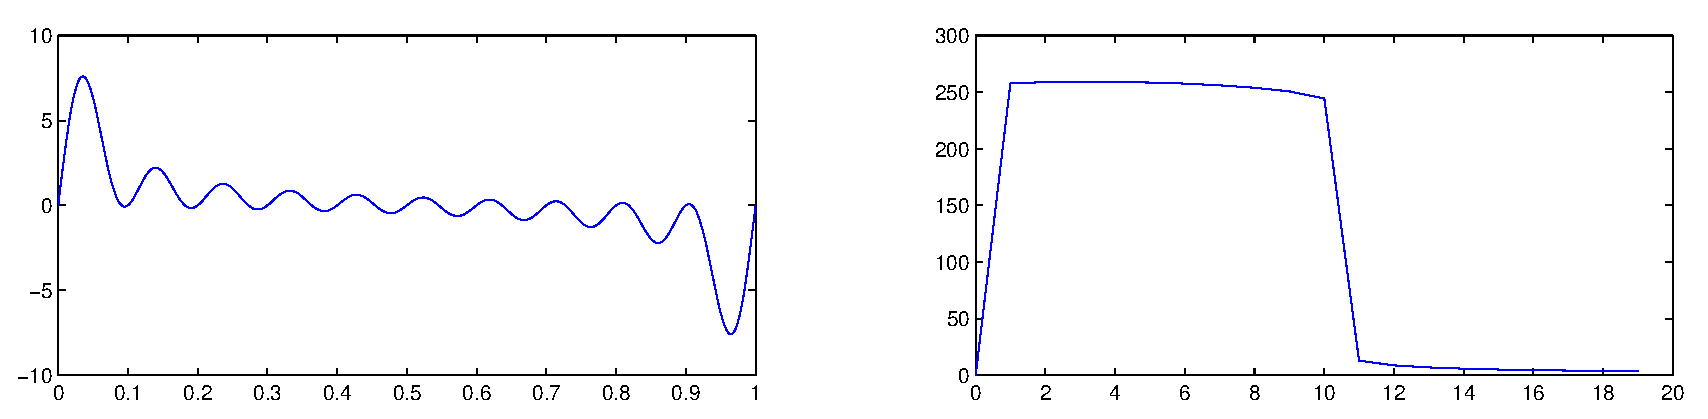
\includegraphics[width=\textwidth, height=0.3\textwidth]{periotriga.eps}
        \caption{Oorspronkelijke functie met $K=256$}
        \label{fig:periotriga}
        \vspace*{1cm}
    \end{subfigure}
    \begin{subfigure}[b]{\textwidth}
        \centering
        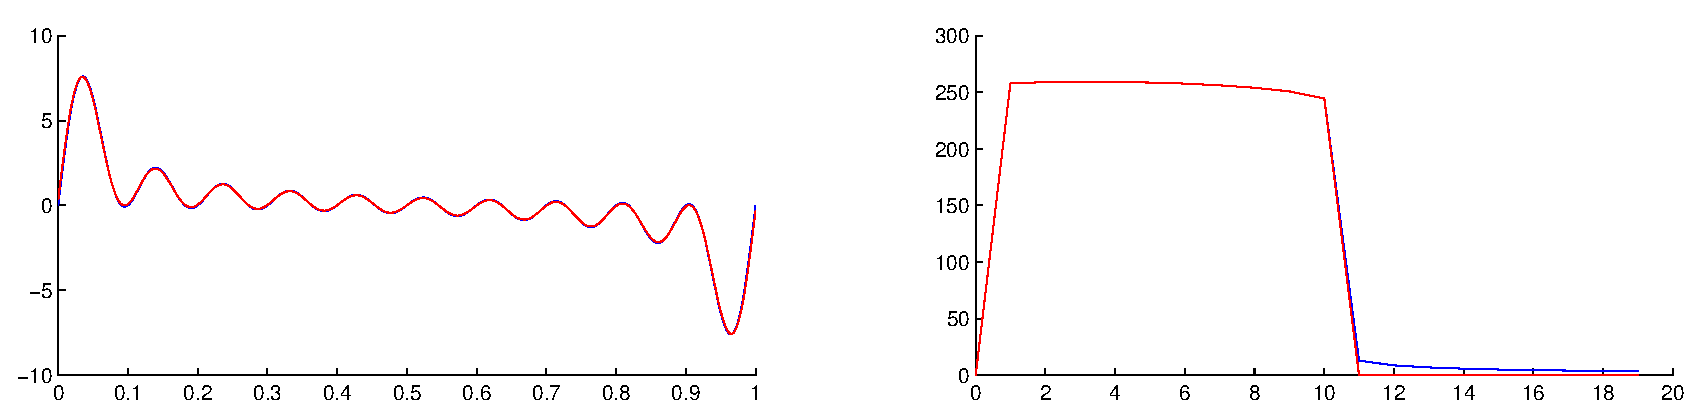
\includegraphics[width=\textwidth]{periotrigb.eps}
        \caption{Benaderende functie met $K=10$}
        \label{fig:periotrigb}
        \vspace*{1cm}
    \end{subfigure}
    \hfill
    \begin{subfigure}[b]{\textwidth}
        \centering
        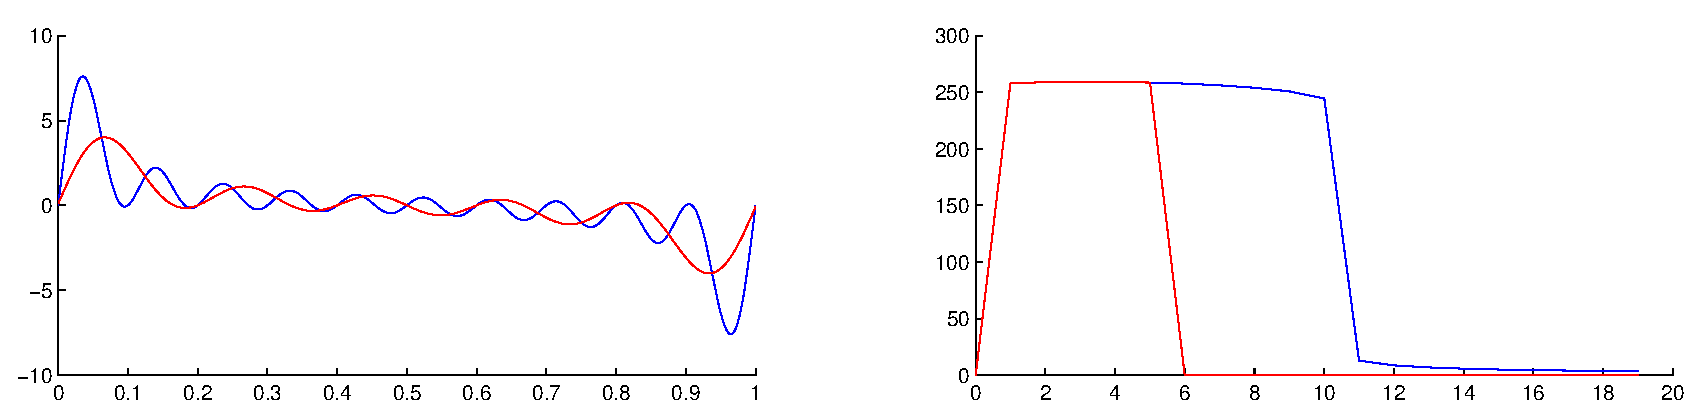
\includegraphics[width=\textwidth]{periotrigc.eps}
        \caption{Benaderende functie met $K=5$}
        \label{fig:periotrigc}
        \vspace*{1cm}
    \end{subfigure}
    \caption{Illustratie van de invloed van de parameter $K$ op de benadering (rood) van een periodieke functie (blauw) met aan de linkerkant de veelterm en aan de rechterkant de FFT van deze veelterm weergegeven over een nuttig domein. ($M = N = 512$)}\label{fig:periotrig}.
\end{figure}
\opgave{8}
In Figuur \ref{fig:periotrigclick} wordt een benadering geconstrueerd voor het $\infty$ teken aan de hand van de functies \textit{click()} en \textit{periotrig(x,K,M)}. In de linkse deelfiguur zijn de oorspronkelijke punten weergegeven die met \textit{click()} zijn getekend. De rechterfiguur toont een periodieke interpolerende en benaderende trigonometrische veelterm voor deze punten.

Aangezien het teken $\infty$ geschreven kan worden als een speciaal geval (met name \textit{het lemniscaat van Gerono}) van de meer algemene \textit{Lissajousfiguur}, is deze benadering uiterst geschikt omdat de parametrisaties bij een \textit{Lissajousfiguur} van de volgende vorm zijn:
\begin{equation}
    \centering
        \begin{cases}
            x=\sin (\alpha t+\delta)\\
            y=\sin (\beta t)
        \end{cases}
\end{equation}
Wanneer in deze vergelijkingen de waarden $\alpha=1$,$\beta=2\alpha=2$ en $\delta=0$ worden genomen, verkrijgt men Figuur \ref{fig:lissajous}.
\begin{figure}
    \centering
    \begin{subfigure}[b]{0.4\textwidth}
        \centering
        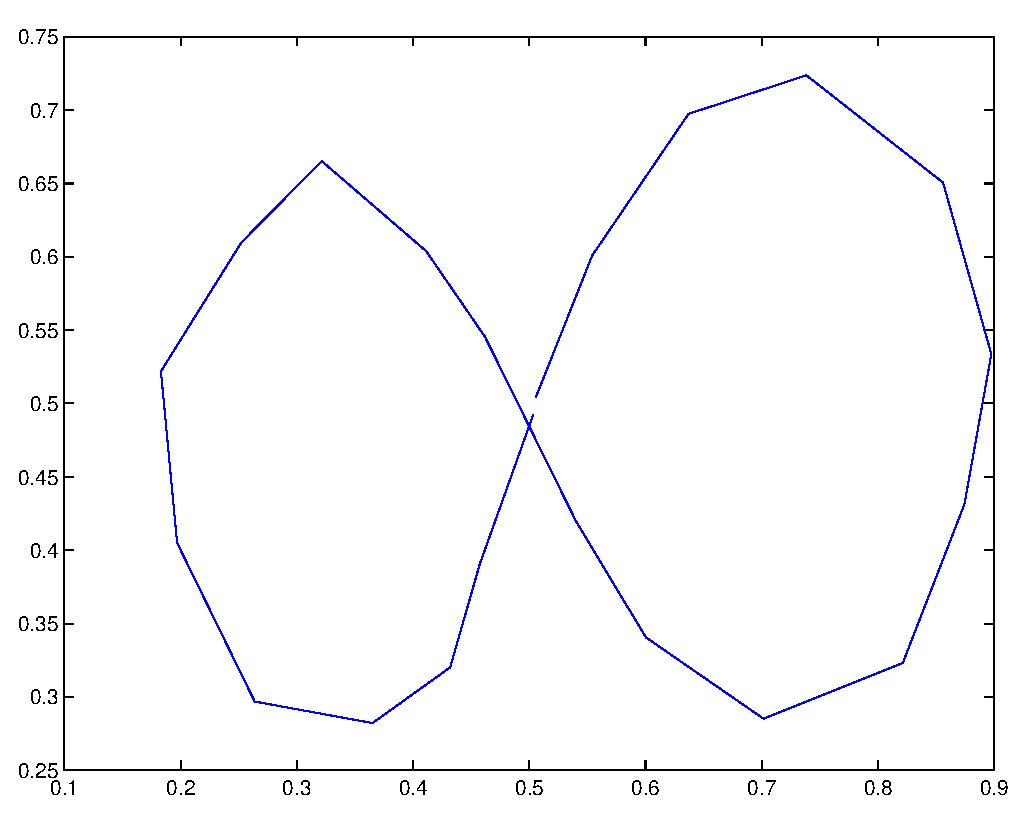
\includegraphics[width=\textwidth]{infclick.eps}
        \caption{Punten met \textit{click()}}
        \label{fig:periotriga}
    \end{subfigure}
    \begin{subfigure}[b]{0.4\textwidth}
        \centering
        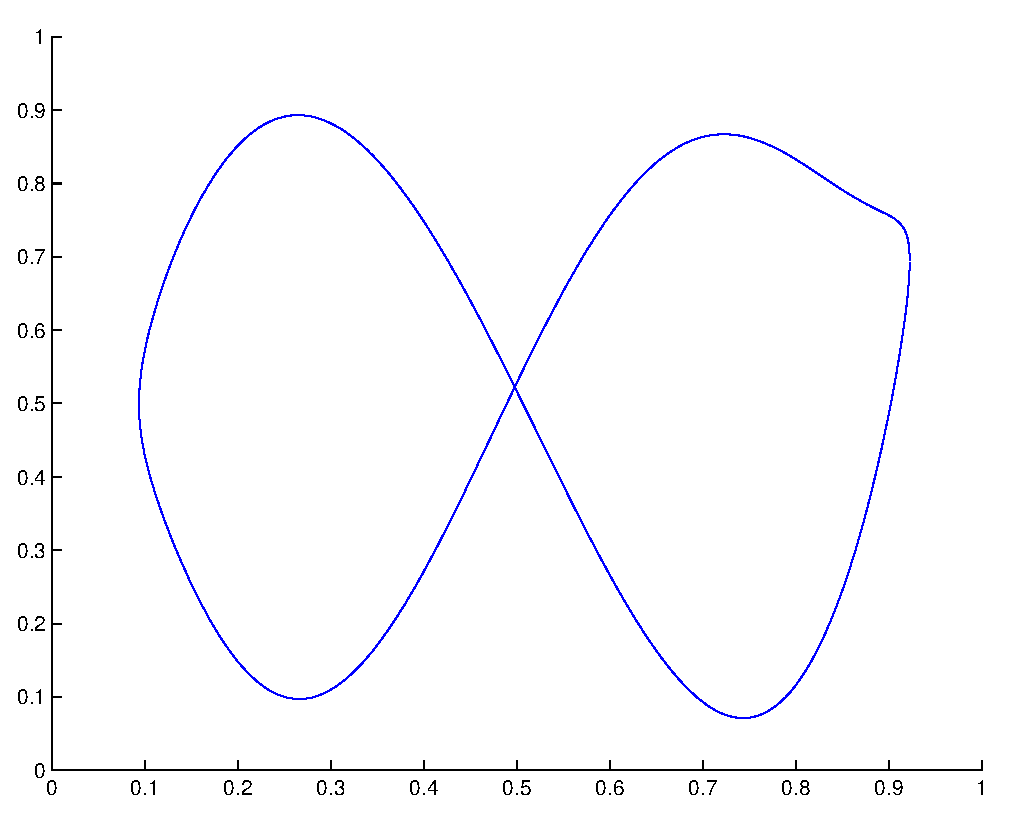
\includegraphics[width=\textwidth]{inftrig.eps}
        \caption{Benaderende functie}
        \label{fig:periotrigb}
    \end{subfigure}
    \hfill
    \caption{$\infty$ teken benaderd}\label{fig:periotrigclick}.
\end{figure}
\begin{figure}
        \centering
        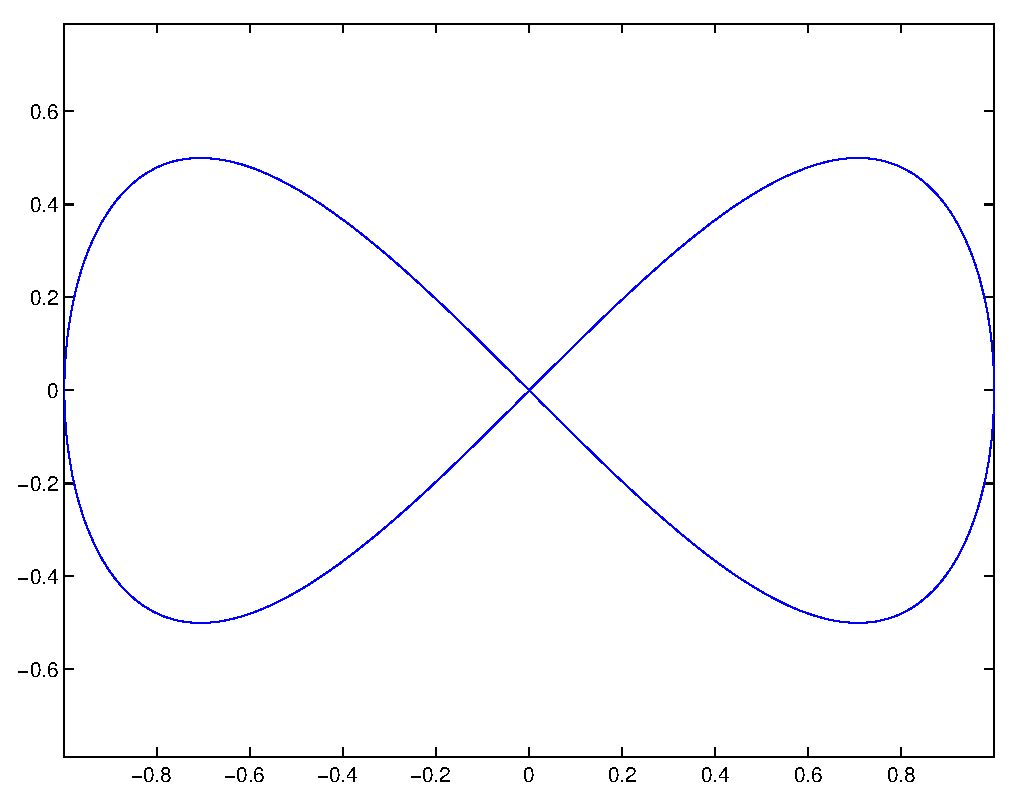
\includegraphics[width=0.85\textwidth]{lissajous.eps}
        \caption{Het $\infty$ teken onder de vorm van een Lissajousfiguur}
        \label{fig:lissajous}
    \end{figure}
\newpage
\section*{Bijlage 1} 
\lstinputlisting{periotrig.m}
\label{bijlage1}
\end{document}